\documentclass[12pt]{article}

% Language setting
% Replace `english' with e.g. `spanish' to change the document language
\usepackage[spanish]{babel}

% Set page size and margins
% Replace `letterpaper' with `a4paper' for UK/EU standard size
\usepackage[letterpaper,top=2cm,bottom=2cm,left=3cm,right=3cm,marginparwidth=1.75cm]{geometry}

% Paquetes
\usepackage{amsmath}
\usepackage{graphicx}
\usepackage{lipsum}
\usepackage{makeidx}
\usepackage{hyperref}
\usepackage[thinlines]{easytable}
\usepackage{listings}
\usepackage{xcolor}
\usepackage{fancyhdr}
\usepackage{verbatim}
\usepackage{parskip}

% Configuración de colores para los enlaces
\hypersetup{
    colorlinks=true,
    linkcolor=black, % Color de los enlaces internos (incluido el índice)
    urlcolor=blue,   % Color de los enlaces externos
    citecolor=blue  % Color de las citas
}

% Estilo para mostrar bonito el código
\definecolor{codegreen}{rgb}{0,0.6,0}
\definecolor{codegray}{rgb}{0.5,0.5,0.5}
\definecolor{codepurple}{rgb}{0.200,0,0.82}
\definecolor{backcolour}{rgb}{0.95,0.95,0.95}

\lstdefinestyle{mystyle}{
    backgroundcolor=\color{backcolour},   
    commentstyle=\color{codegreen},
    keywordstyle=\color{magenta},
    numberstyle=\tiny\color{codegray},
    stringstyle=\color{codepurple},
    basicstyle=\ttfamily\footnotesize,
    breakatwhitespace=false,         
    breaklines=true,                 
    captionpos=b,                    
    keepspaces=true,                 
    numbers=left,                    
    numbersep=5pt,                  
    showspaces=false,                
    showstringspaces=false,
    showtabs=false,                  
    tabsize=2
}
\lstset{style=mystyle}

\makeindex

% Encabezado
\pagestyle{fancy}
% Set the header and footer for Even
% pages but omit the zone (L, C or R)
\fancyhead[L]{\leftmark}
\fancyhead[R]{Análisis de Algoritmos - 2024}
\fancyfoot[L]{\href{https://github.com/garaneda21/Particionamiento-De-Palindromos}{Código en GitHub}}
\fancyfoot[C]{}
\fancyfoot[R]{Página \thepage} % Número de página en la derecha

\setlength{\headheight}{30pt} % Ajuste de altura del encabezado
\setlength{\footskip}{15pt}   % Ajusta la distancia entre el pie de página y el texto principal



\begin{document}

\begin{titlepage}
    \centering
    \vspace*{1cm}

    \Huge
    \textbf{Informe Trabajo n.º 2 Análisis de Algoritmos}

    \vspace{1cm}

    
\includegraphics[width=0.5\textwidth]{Logo_UTEM.png}

    \vspace{0.1cm}

    \Large
    

\begin{flushleft}

    \textbf{\underline{Integrantes:}}\\
    Gerardo Araneda\\
    Andrés Gómez\\

    \vspace{0.6cm}

    \textbf{\underline{Asignatura:}}\\
    Análisis de Algoritmos

    \vspace{0.6cm}

    \textbf{\underline{Sección:}}\\
    301
    
    \vspace{0.6cm}

    \textbf{\underline{Profesor:}}\\
    Luis Herrera Becerra
  
\end{flushleft}

\end{titlepage}

\tableofcontents
\newpage
% AQUI EMPIEZA TODO

\section{Introducción}

\vspace{1em}
\begin{minipage}{1\linewidth}
    \centering
    Link al código en GitHub: 
    \url{https://github.com/garaneda21/Particionamiento-De-Palindromos}
\end{minipage}

En la informática y ciencias computacionales, el análisis de algoritmos desempeña un papel importante
al evaluar el rendimiento y la eficiencia de los algoritmos utilizados para resolver problemas
específicos. Uno de los paradigmas más destacados en este campo es la programación dinámica, técnica que permite resolver problemas complejos dividiéndolos en subproblemas más simples y
almacenando las soluciones de estos subproblemas para evitar recálculos innecesarios.

En este trabajo se hará el análisis del problema de particionamiento de palíndromos. Este problema
consiste en dividir una cadena de caracteres en el menor número posible de subcadenas que sean
palíndromos (secuencias que se leen igual de adelante hacia atrás y viceversa). \\

Ejemplo 1: \\\\
Cadena: \textbf{ababbbabbababa} \\\\
Particionamiento de palíndromos: \textbf{a — babbbab — b — aba} \\\\
Ejemplo 2: \\\\
Cadena: \textbf{geek} \\\\
Particionamiento de palíndromos: \textbf{g — ee — k} \\\\
Explicación: Necesitamos hacer un mínimo de 2 cortes, es decir, ”g — ee — k”. \\

En este informe, se presentan dos algoritmos para abordar el problema de particionamiento de 
palíndromos, los cuales se nombran como Algoritmo A y Algoritmo B. para estos algoritmos sé realiza un análisis para comprobar sus complejidades asintóticas, donde se llega a para el algoritmo A una complejidad de $O(n^3)$ y para el Algoritmo B $O(n^2)$. Luego se creó un programa que mide los tiempos de ejecución de estos algoritmos para representar gráficamente la relación entre largo de la entrada vs. tiempo.

A modo de hipótesis, se espera que los gráficos muestren una curva que tienda al límite superior establecido por la función asintótica correspondiente para cada algoritmo y también se espera que el algoritmo con un límite inferior presente tiempos de ejecución más rápidos.

\newpage
\section{Metodología}

Los Algoritmos se implementaron con ayuda de los artículos de GeeksforGeeks, agradecimientos respectivos a sus creadores \cite{geeksforgeeks}

\subsection{Solución de Enfoque Recursivo}

Las soluciones siguientes plantean optimizar la solución recursiva de este problema, cuya implementación no se explorará en este informe. Esta solución realiza todas las particiones en la cadena de texto hasta encontrar una que sea palíndromo, en ese caso realiza el corte y se lo suma a las siguientes particiones.

\begin{figure}[ht]
    \centering
    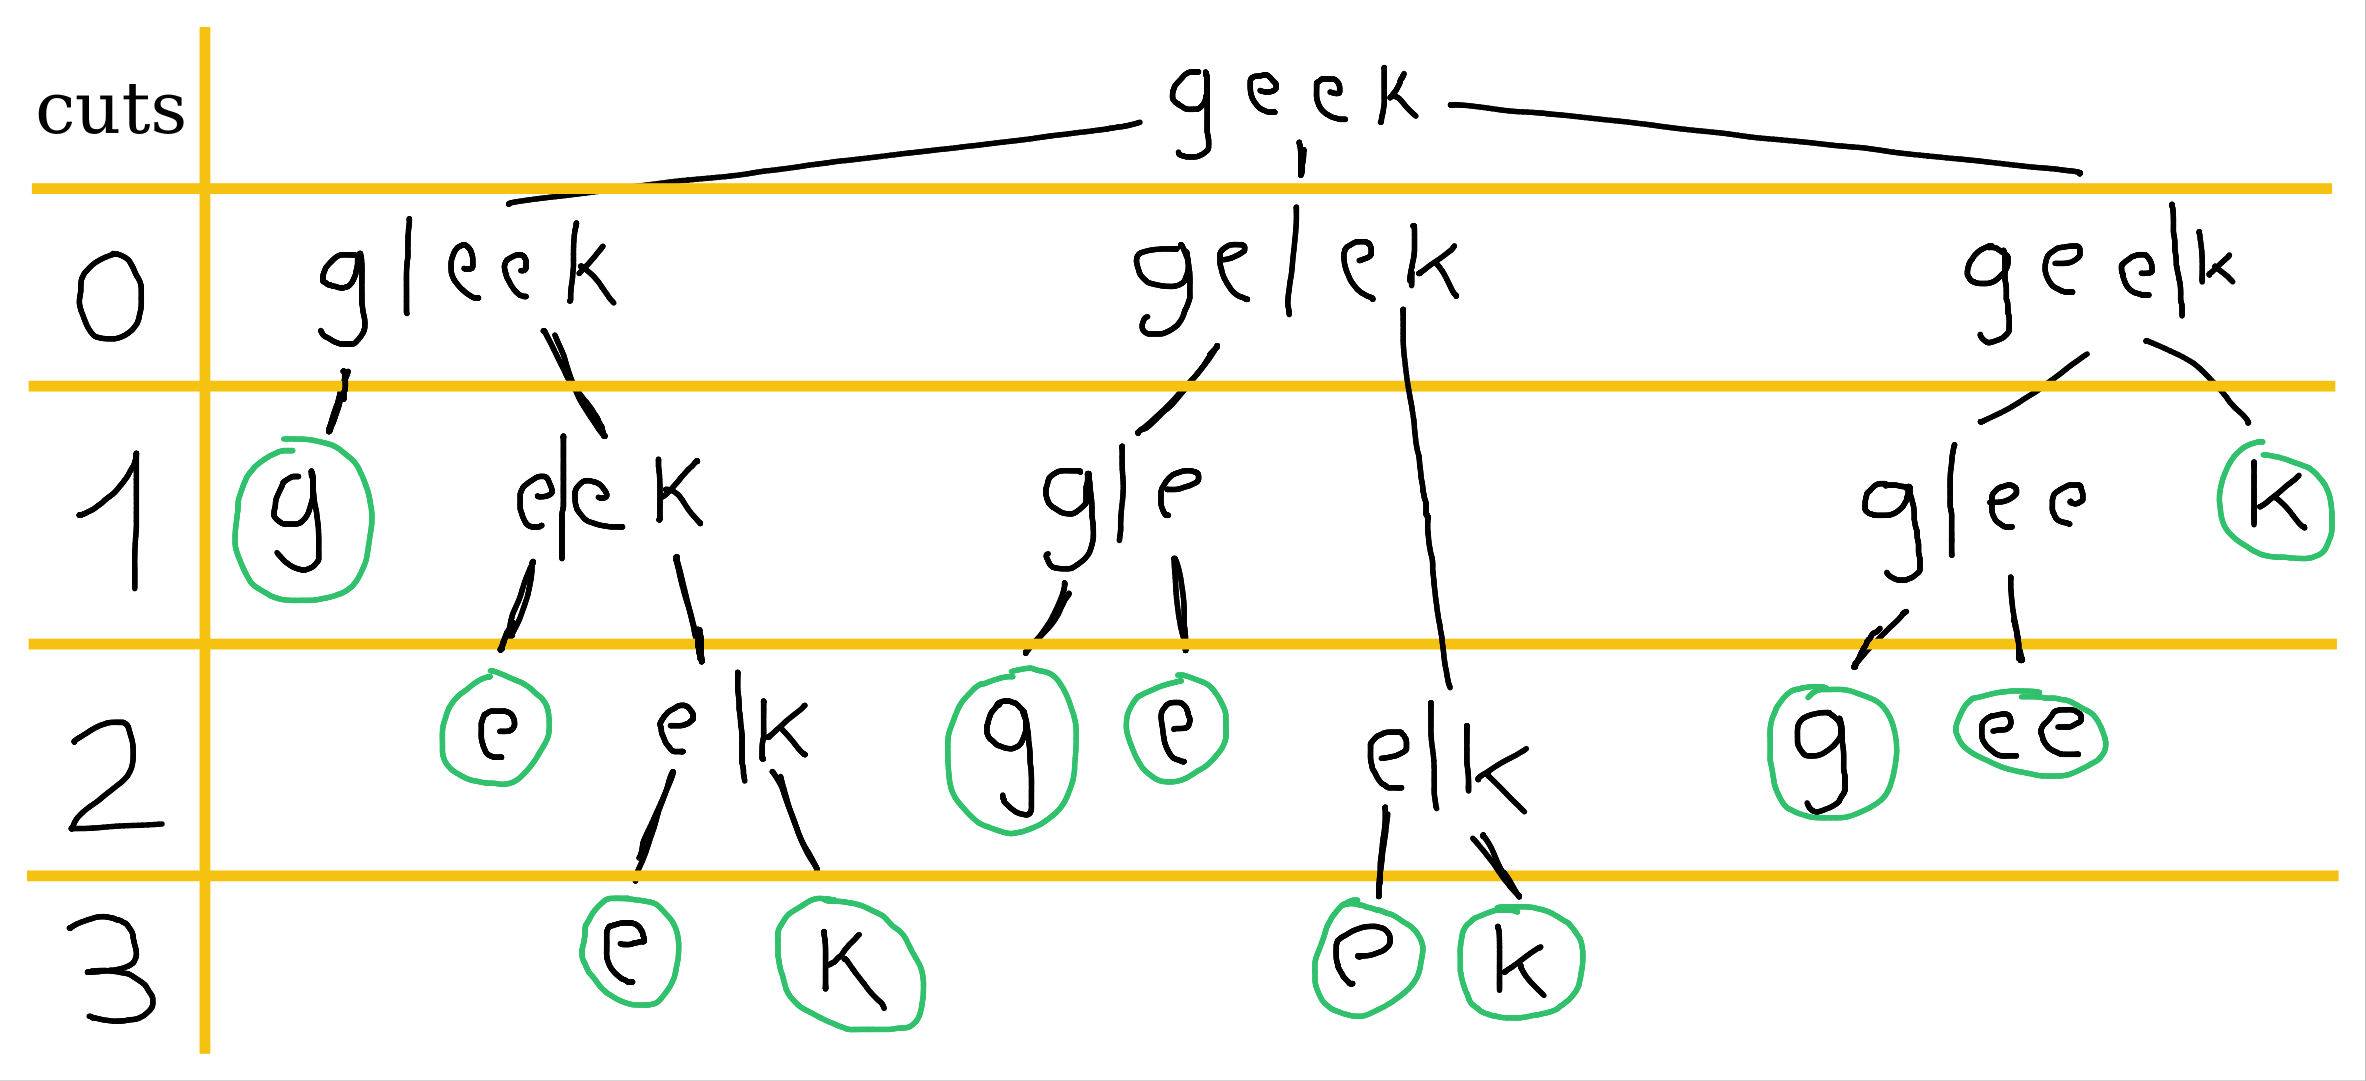
\includegraphics[width=\textwidth]{rec.png}
    \caption{Árbol de la solución recursiva para cadena geek}
\end{figure}

En la Figura 1, se encuentra como se desarrolla esta solución por el algoritmo,
donde para cada subcadena, si se comprueba que no es un palíndromo, se realiza un nuevo corte hasta encontrar otro palíndromo o llegar a un solo carácter. Como al realizar un corte nos quedan 2 subcadenas, para una cadena de largo $n$ se observa que $T(n) = O(2^n)$ dado el branching factor de 2.

\subsection{Algoritmo A, Solución de Programación Dinámica O(n³)}

Dada una Cadena $[0...n-1]$ con $n$ el largo de la cadena, esta solución consiste en usar dos Matrices, $C$, la cual guarda el número de cortes mínimos necesarios para particionar la Cadena y $P$, la cual contendrá si la subcadena[i,j] es o no un palíndromo.

Esta solución se va construyendo de forma Bottom-up, y es similar al problema de parentización de matrices
\newpage

La implementación realizada en el lenguaje Python es la siguiente:


% Monstrar Código
\begin{figure}[h]
    \centering
    \lstinputlisting[language=Python]{rec2.py}
    \caption{Implementación en Programación dinámica $O(n^3)$}
\end{figure}

La función palPart recibe una cadena para hacer las particiones, se obtiene su largo y Se Inicializan las matrices $C$ y $P$. Este algoritmo ordena la cadena y sus subcadenas como se muestra en la Figura 3, abarcando todos los cortes posibles donde los índices $i, j$ representa el subarreglo[$i,j$] (Ej. subarreglo$[0,3] = $ gee):

\begin{figure}[h]
    \centering
    \begin{TAB}(e,1cm,1cm){c|c|c|c|c|}{c|c|c|c|c|}
        i/j & j=0 & j=1 & j=2 & j=3 \\ 
        i=0 & g & ge  & gee  & geek \\
        i=1 & / & e   & ee   & eek  \\
        i=2 & / & /   & e    & ek   \\
        i=3 & / & /   & /    & k   
    \end{TAB}
    \caption{como el algoritmo ordena la cadena}
\end{figure}

Los valores donde $j<i$ no se toman en cuenta, ya que no tienen sentido.

Dada la matriz de la Figura 3, las matrices $C$ y $P$ tienen esta forma: \newpage

% Matrices C y P
\vspace{1em}
\begin{minipage}{0.45\linewidth}
    \centering
    \textbf{Matriz C} \\[1em]
    \begin{TAB}(e,1.25cm,1.25cm){|c|c|c|c|}{|c|c|c|c|}
        0 & 0  & 0  & 0 \\
        / & 0  & 0  & 0 \\
        / & /  & 0  & 0 \\
        / & /  & /  & 0 
    \end{TAB}
\end{minipage}
\hfill
\begin{minipage}{0.45\linewidth}
    \centering
    \textbf{Matriz P} \\[1em]
    \begin{TAB}(e,1.25cm,1.25cm){|c|c|c|c|}{|c|c|c|c|}
        False & False & False & False \\
        /     & False & False & False \\
        /     & /     & False & False \\
        /     & /     & /     & False    
    \end{TAB}
\end{minipage}
\vspace{2em}

Ahora, como el algoritmo usa la forma Bottom-up y sabiendo que las cadenas de largo 1 son palíndromo, en la línea 7 se inicia marcando estas cadenas como true en la Matriz $P$ y 0 en la Matriz $C$, ya que no es necesario realizar cortes, quedando de esta forma

% Matrices C y P
\vspace{1em}
\begin{minipage}{0.45\linewidth}
    \centering
    \textbf{Matriz C} \\[1em]
    \begin{TAB}(e,1.25cm,1.25cm){|c|c|c|c|}{|c|c|c|c|}
        \textbf{0} & 0  & 0  & 0 \\
        / & \textbf{0}  & 0  & 0 \\
        / & /  & \textbf{0}  & 0 \\
        / & /  & /  & \textbf{0} 
    \end{TAB}
\end{minipage}
\hfill
\begin{minipage}{0.45\linewidth}
    \centering
    \textbf{Matriz P} \\[1em]
    \begin{TAB}(e,1.25cm,1.25cm){|c|c|c|c|}{|c|c|c|c|}
        \textbf{True}  & False & False & False \\
        /     & \textbf{True}  & False & False \\
        /     & /     & \textbf{True}  & False \\
        /     & /     & /     & \textbf{True}    
    \end{TAB}
\end{minipage}
\vspace{2em}

Ahora, en la línea 11, usando el primer ciclo for se comienza a recorrer el resto de los subarreglos de forma Bottom-up, partiendo con los de largo 2 hasta los de largo n, en las matrices serían todas las diagonales.
Después, en el segundo ciclo for se recorre cada una de las subcadenas analizando las siguientes condiciones:
\begin{enumerate}
    \item Los Caracteres de las esquinas son iguales (para formar el palíndromo)
    \item La subcadena aparece en la Matriz P como palíndromo (Programación Dinámica) o si la subcadena es de largo 2 (no contiene subcadenas)
\end{enumerate}

Si se cumplen estas condiciones, se pasa a la línea 16 donde la subcadena es un palíndromo, por lo que se añade a la matriz P y se marca que no necesita cortes en la matriz C
Si no se cumplen estas condiciones, se pasa a la línea 19 donde la subcadena no es un palíndromo y se procede a comprobar con el resto para obtener el que tenga el mínimo número de cortes dándole a este un número infinito de cortes $C[i,j] = \infty$. Aquí se entra al tercer ciclo for, donde se hace el cálculo respectivo usando la misma fórmula que en el problema de parentización de matrices.

$$\min\{M[i,j], M[i,k] + M[k+1,j] + \text{costo de la multiplicación} \}$$

En este caso, sería el costo mínimo entre la subcadena actual C[i,j] el cual está marcado como infinito, y el costo de la subcadena C[i,k] más la subcadena C[k+1,j] más 1, que es el corte realizado dado que no es un palíndromo.

$$\min\{C[i,j], C[i,k] + C[k+1,j] + 1 \}$$

el bucle sigue comprobando el resto de cortes hasta obtener el número mínimo para esa subcadena. Finalmente, se guarda el valor mínimo en la matriz $C$ y se continúa con la siguiente iteración

Para la cadena "geek", las matrices quedan de la siguiente forma al terminar el algoritmo:

% Matrices C y P
\vspace{1em}
\begin{minipage}{0.45\linewidth}
    \centering
    \textbf{Matriz C} \\[1em]
    \begin{TAB}(e,1.25cm,1.25cm){|c|c|c|c|}{|c|c|c|c|}
        0 & 1  & 1  & 2 \\
        / & 0  & 0  & 1 \\
        / & /  & 0  & 1 \\
        / & /  & /  & 0 
    \end{TAB}
\end{minipage}
\hfill
\begin{minipage}{0.45\linewidth}
    \centering
    \textbf{Matriz P} \\[1em]
    \begin{TAB}(e,1.25cm,1.25cm){|c|c|c|c|}{|c|c|c|c|}
        True  & False & False & False \\
        /     & True  & True  & False \\
        /     & /     & True  & False \\
        /     & /     & /     & True    
    \end{TAB}
\end{minipage}
\vspace{2em}

Donde finalmente, la función retorna el valor $C[0,n-1]$ que es el mínimo número de cortes calculado, en este caso siendo igual a 2 cortes, g|ee|k.

Esta función al tener 3 ciclos for anidados, Se obtiene la Complejidad de $O(n^3)$

$$\text{Complejidad Algorimto A: } T(n) = O(n^3)$$

\subsection{Algoritmo B, Solución de Programación Dinámica O(n²)}

Dada una Cadena $[0...n-1]$ con $n$ el largo de la cadena, esta solución consiste en usar una Matriz $P$ la cual contiene si la subcadena[i,j] es o no un palíndromo, y un arreglo minCutDP[n-1], el cual contiene el número mínimo de cortes para cada una de las subcadenas.

Esta solución utiliza los sufijos que comienzan desde una posición j hasta i de la cadena, que son palíndromos, donde $(1 \leq j \leq i \leq n-1)$, de esta forma, por cada sufijo palíndromo se hace un corte y se suma con el número mínimo de cortes del resto de la subcadena.

\newpage
La implementación realizada en el lenguaje Python es la siguiente:

% Monstrar Códigos
\begin{figure}[htbp]
    \centering
    \lstinputlisting[language=Python]{dp3-generarPalindromo.py}
    \lstinputlisting[language=Python]{dp3-minCutDP.py}
    \caption{Función auxiliar generarPalindromo y Función minCutDP, Implementación en Programación dinámica $O(n^2)$}
\end{figure}

Usando nuevamente el ejemplo de la cadena "geek", la función minCutDP recibe una cadena para hacer las particiones, se obtiene su largo $n$ y usando la función auxiliar generarPalindromo, se procede a inicializar la matriz $P$ de inmediato con las subcadenas[i,j] que sean palíndromos, quedando de la siguiente forma: 

% Matriz P
\vspace{1em}
\begin{minipage}{\linewidth}
    \centering
    \textbf{Matriz P} \\[1em]
    \begin{TAB}(e,1cm,1cm){|c|c|c|c|}{|c|c|c|c|}
        True  & False & False & False \\
        /     & True  & True  & False \\
        /     & /     & True  & False \\
        /     & /     & /     & True    
    \end{TAB}
\end{minipage}
\vspace{2em}

Luego se inicializa el arreglo minCortesDP[] que contiene el número de cortes para cada subcadena de largo i, con la posición minCortesDP[0] = 0, ya que las subcadenas de largo 1 son palíndromos. la representación de este arreglo es la siguiente:

% Arreglo
$$ \text{minCortesDP} = \begin{bmatrix}
0 & \infty & \infty & \infty 
\end{bmatrix}  $$

Ahora, el primer bucle donde se irá recorriendo la cadena desde la posición 1 hasta el largo $n$, analizando cada subcadena. Ahora se comprueba si la subcadena actual es palíndromo, si es así no se necesitan hacer cortes y se marcaría como 0 en la posición $i$ del arreglo minCortesDP. Si no, se entra al segundo bucle donde recorren los sufijos de la subcadena desde la posición actual i hasta 0 en reversa para ver si son palíndromos, el primer sufijo siempre será palíndromo porque la posición $i = j$ es de largo 1. Aquí se realiza un corte y se suma con el número mínimo de cortes de la subcadena anterior y se toma este como referencia para el resto de cortes. luego para los sufijos donde $j < i$ se comprueban si son palíndromos para seguir minimizando los cortes hasta recorrer totalmente la subcadena sufijos.

Una vez terminadas todas las iteraciones, se retorna el valor minCortesDP[n-1] que es el número mínimo de cortes de toda la cadena. el arreglo de minCortesDP[n-1] terminaría de esta forma:
% Arreglo
$$ \text{minCortesDP} = \begin{bmatrix}
0 & 1& 1 & \textbf{2} 
\end{bmatrix}  $$

en este caso, se retorna el valor 2, que es el mínimo número de cortes calculado: g|ee|k

En comparación con la solución de la sección anterior (2.2), este contiene solo dos bucles for anidados, teniendo una complejidad de $O(n^2)$, mucho mejor que la anterior $O(n^3)$ para una entrada $n$ muy grande.

$$\text{Complejidad Algorimto B: } T(n) = O(n^2)$$

\subsection{Medición de tiempos de ejecución de ambos algoritmos}
Para comprobar de manera práctica las complejidades de los algoritmos, se generaron 1,000 palabras de forma aleatoria con una longitud entre $1$ y 500 caracteres. Luego, utilizando Python, se creó un programa que reciba cada palabra y la procese con cada algoritmo, calculando su tiempo de ejecución para cada palabra. Estos tiempos se registran en un archivo en formato .CSV, que posteriormente se puede abrir con un software de hojas de cálculo como Microsoft Excel para generar un gráfico que muestre la relación entre la longitud de la palabra y el tiempo de ejecución.


\section{Resultados}

Al ejecutar el programa creado, este muestra el siguiente output (output completo en repositorio de GitHub):

\begin{verbatim}
$ python main.py

1 : Tiempo A:  4.240746974945068 seg     Tiempo B: 0.028652191162109375
2 : Tiempo A:  0.5069446563720703 seg    Tiempo B: 0.004831552505493164
3 : Tiempo A:  0.6496925354003906 seg    Tiempo B: 0.006289005279541016

...

998 : Tiempo A:  1.4912116527557373 seg  Tiempo B: 0.012072086334228516
999 : Tiempo A:  2.0959622859954834 seg  Tiempo B: 0.014597177505493164
1000 : Tiempo A:  1.2563939094543457 seg  Tiempo B: 0.01026010513305664
Archivo tiempos.csv Creado con Exito.
\end{verbatim}

El archivo tiempos.csv generado, al abrirlo en un software de hojas de calculo muestra lo siguiente: 

\begin{figure}[ht]
    \centering
    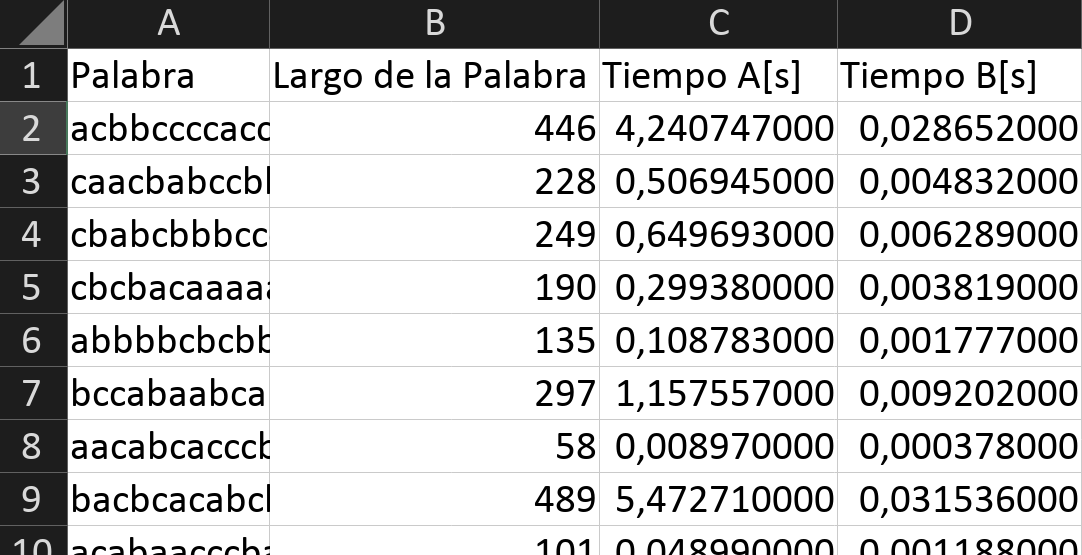
\includegraphics[width=0.7\textwidth]{excel-csv.png}
    \caption{Contenido del archivo tiempos.scv generado por el programa}
\end{figure}

Los tiempos de ambos algoritmos se convirtieron a milisegundos, y se crearon los gráficos del Largo de la Palabra vs. Tiempo de los Algoritmos (Figuras 6, 7 y 8).

\begin{figure}[htbp]
    \centering
    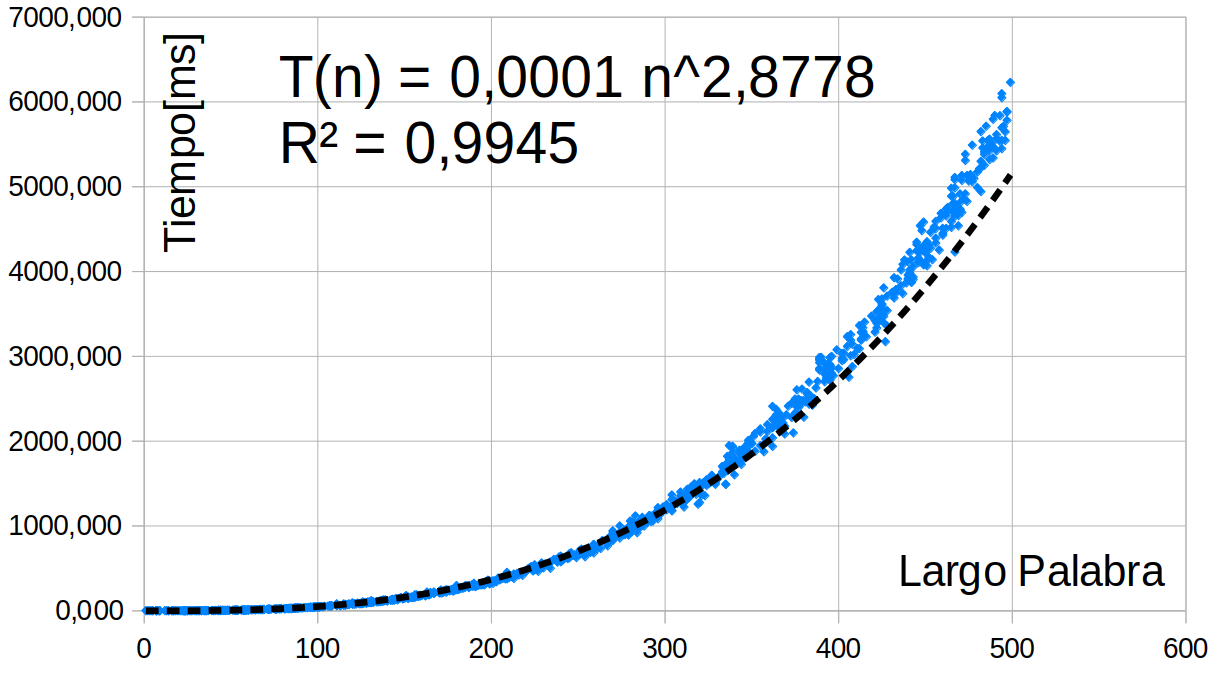
\includegraphics[width=\textwidth]{Grafico1.png}
    \caption{Gráfico Largo de la Palabra vs. Tiempo del Algoritmo A}
\end{figure}

\begin{figure}[htbp]
    \centering
    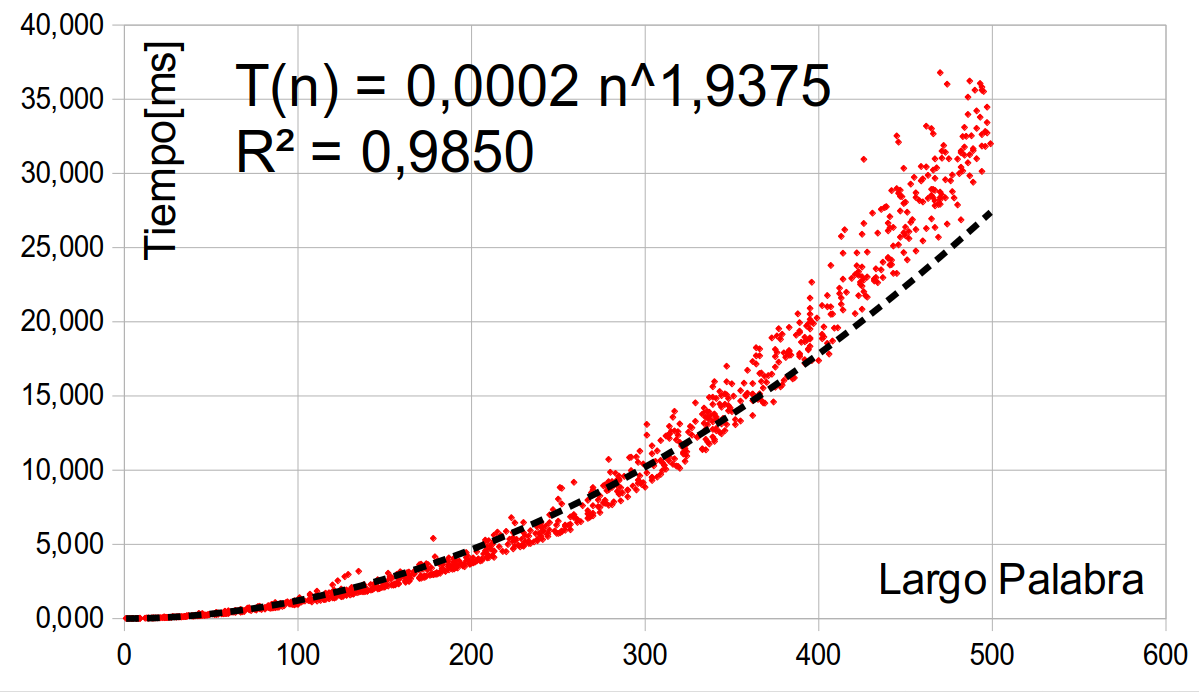
\includegraphics[width=\textwidth]{Grafico2.png}
    \caption{Gráfico Largo de la Palabra vs. Tiempo del Algoritmo B}
\end{figure}

\begin{figure}[htbp]
    \centering
    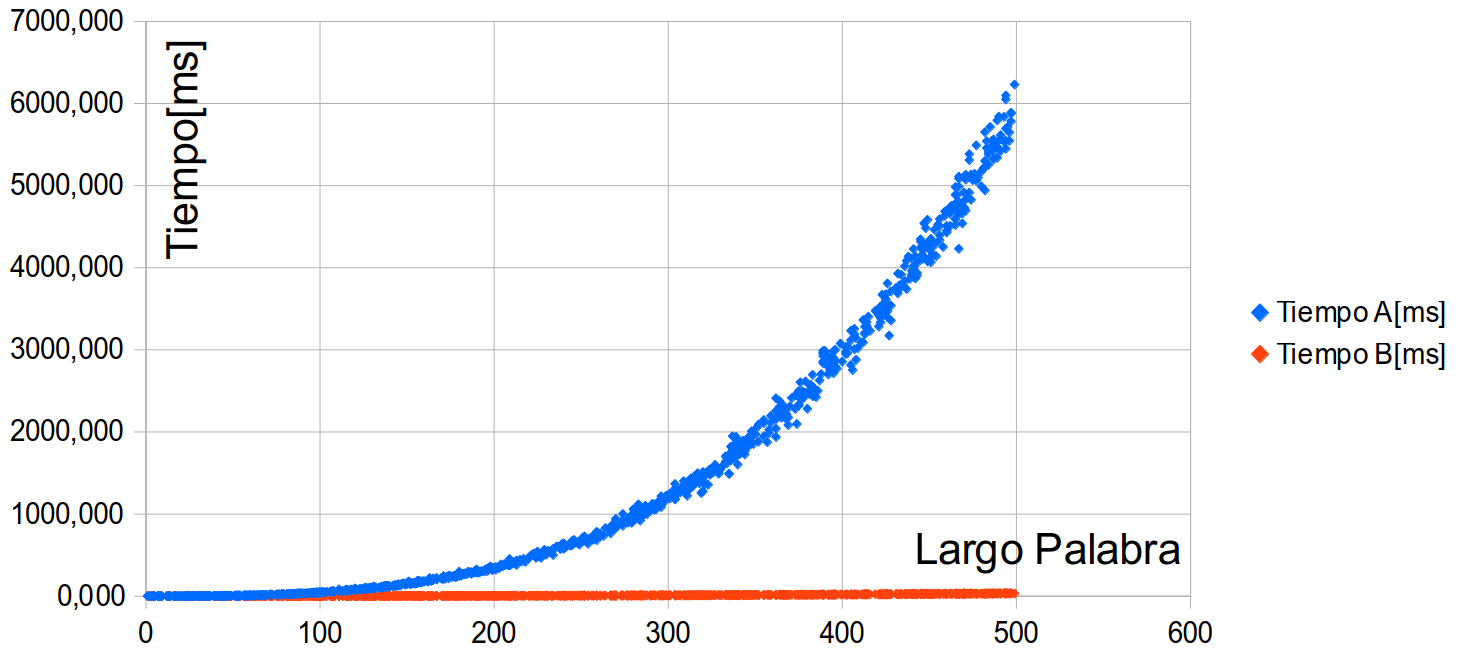
\includegraphics[width=\textwidth]{Grafico3.png}
    \caption{Gráfico Largo de la Palabra vs. Tiempo del Algoritmo A (azul) y B (rojo)}
\end{figure}

\newpage
En estos gráficos se incluyó la linea de tendencia para obtener la función correspondiente a la que tienden los valores, las funciones fueron las siguientes:

$$\text{Algoritmo A}: T(n) = 0,0001n^{2,8778}$$

$$\text{Algoritmo B}: T(n) = 0,0002n^{1,9375}$$

\newpage
\section{Conclusiones}

\subsection{Análisis de Resultados}

En los gráficos se puede apreciar como para una entrada muy grande (Largo de las palabras), el tiempo de ejecucion escala de acuerdo a la complejidad del algoritmo.

Además, en el gráfico de la figura 8, se aprecia que el Algoritmo B es significativamente más rápido que el Algoritmo A, donde el Algoritmo B no supera el segundo de ejecución en las pruebas realizadas.

\subsubsection{Algoritmo A}
En el gráfico de la figura 6, se obtuvo la funcion $T(n) = O(n^{2,8778})$ y del análisis asintótico se puede decir que

$$O(n^{2,8778}) = O(n^3)$$

En la metodología al analizar este algoritmo se dijo que tenia una complejidad de $O(n^3)$ por lo que se cumple nuestra hipótesis planteada.

\subsubsection{Algoritmo B}
En el gráfico de la figura 7, se obtuvo la funcion $T(n) = O(n^{1,9375})$ y del análisis asintótico se puede decir que

$$O(n^{1,9375}) = O(n^2)$$

En la metodología al analizar este algoritmo se dijo que tenia una complejidad de $O(n^2)$ por lo que se cumple nuestra hipótesis planteada.

\subsection{Conclusiones Generales}

El análisis y la comparación de los tiempos de ejecución de ambos algoritmos han demostrado la validez de nuestras hipótesis iniciales sobre sus complejidades. El Algoritmo B, con una complejidad de $O(n^2)$, se mostró significativamente más eficiente que el Algoritmo A, cuya complejidad es $O(n^3)$. Esto es evidente en los gráficos, donde el Algoritmo B tiene tiempos de ejecución muy bajos.

Los resultados obtenidos demuestran la importancia de considerar la complejidad algorítmica en el diseño de algoritmos, especialmente cuando se trata de manejar grandes volúmenes de datos. Lograr implementar un algoritmo con una complejidad más baja y utilizando las técnicas vistas en clase como la programación dinámica utilizada en este trabajo puede llevar a mejoras significativas en el rendimiento y la eficiencia.

% Bibliografia / Referencias

\addcontentsline{toc}{section}{Referencias}
\begin{thebibliography}{}

\bibitem{geeksforgeeks}
GeeksforGeeks. (2024, marzo 8). Palindrome partitioning. \url{https://www.geeksforgeeks.org/palindrome-partitioning-dp-17/}
\bibitem{textbook}
Cormen, T. H., Leiserson, C. E., Rivest, R. L., \& Stein, C. (2022). Introduction to Algorithms, fourth edition. MIT Press.

\end{thebibliography}

\end{document}